\documentclass{article}
\usepackage{graphicx}
\usepackage[margin=1.5cm]{geometry}
\usepackage{amsmath}

\begin{document}
\twocolumn

\title{Wednesday warm-up: unit analysis and vectors}
\author{Prof. Jordan C. Hanson}

\maketitle

\section{Unit Analysis, Vectors}

\begin{enumerate}
\item Suppose a track runner completes a 1600 meter run in 275 seconds.  (a) What is the average speed of the runner in meters per second? (b) Convert this to miles per minute (1 mile is 1.6 km). \\ \vspace{2cm}
\item Accerlation is defined as the rate of change in velocity.  If a train starts at rest, and accelerates to 30 km hr$^{-1}$ in 40 seconds,  what is the acceleration in m s$^{-2}$? 
\begin{itemize}
\item A: 2.0 m s$^{-2}$
\item B: 0.2 m s$^{-2}$
\item C: 2.0 m s$^{-1}$
\item D: 0.2 m s$^{-1}$
\end{itemize}
\item A barge is pulled by the two tugboats shown in Fig. \ref{fig:1}. The right tugboat pulls with a force of 4000 Newtons, 15 degrees away from the line AB.  The left tugboat pulls with a force of 5000 Newtons, 12 degrees away from the line AB.  (a) Using trigonometry, break each force into x and y components, and list them below.  (b) What is the total force (as a vector) in Newtons? \\ \vspace{3cm}
\item (a) In the previous exercise, at what angle does the total force pull? \\ \vspace{3cm}
\item One lb (pound) of force is 4.448 Newtons.  Convert the total force from Fig. \ref{fig:1} to lbs (pounds).
\end{enumerate}

\begin{figure}[ht]
\centering
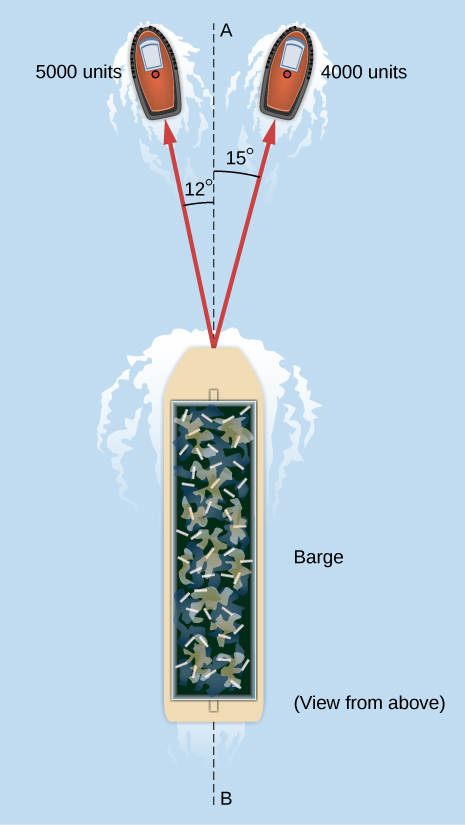
\includegraphics[width=0.45\textwidth]{figures/boat.jpeg}
\caption{\label{fig:1} The barge is pulled by two tugboats, and the tensions in the ropes are described by two vectors.}
\end{figure}

\end{document}
